\documentclass{beamer}

\usepackage[francais]{babel}	% Pour le français
\usepackage[utf8]{inputenc}		% Pour l'utf8
\usepackage[T1]{fontenc}		% Pour le codage latin
\usepackage{helvet}				% Police helvet
\usepackage{hyperref}			% Lien externe
\usepackage{listings}   % code source
\usepackage{minted}

\usetheme{Warsaw}				% Thème Warsaw

\title{Environnement de développement avec Vagrant et Docker}
\author{Maxence Bothorel, Thibaut Crouvezier}
\institute{Licence professionnelle ASRALL,\\
    IUT Nancy Charlemagne,\\
    Nancy}
\date{22/01/2015}

\AtBeginSection[]{
    \begin{frame}
        \frametitle{Sommaire}
        \tableofcontents[currentsection, hideothersubsections]{}
    \end{frame}
}

\begin{document}

    \begin{frame}
        \maketitle{}
    \end{frame}
    	
    \section{Introduction}
    	
    \begin{frame}
        Intro
    \end{frame}
    
    \section{Vagrant}
    \subsection{Introduction}
    
    \begin{frame}{Vagrant}
        \begin{center}
            
\includegraphics[scale=0.1]{images_rapport/vagrant_logo.jpg}
        \end{center}
        \begin{itemize}
            \item{Développer en Ruby sous licence MIT}
            \item{Créé en 2010 par Mitchell Hashimoto}
            \pause{}
            \item{Utilise des machines virtuelles}
            \item{Public cible : Les développeurs}
        \end{itemize}
    \end{frame}

    \subsection{Utilisation basique}
    \begin{frame}{Utilisation}
        \begin{itemize}
            \item{vagrant init hashicorp/trusty64}
            \item{vagrant up}
            \item{ssh}
        \end{itemize}
        \pause{}
        \begin{block}{Vagrantfile}
            Les Vagrantfile sont les fichiers de configurations. Vagrant va chercher le Vagrantfile en remontant l'arborescence.
        \end{block}
    \end{frame}

    \subsection{Configuration}
    \begin{frame}{Vagrantfile}
        Il existe plusieurs Vagrantfiles. Ils sont tous lus dans un certain ordre :
        \begin{enumerate}
            \item{Le Vagrantfile téléchargé avec la machine.}
            \item{Un Vagrantfile dans le soddier /home/user/.vagrant.d.}
            \item{Le Vagrantfile créé lors de la commande vagrant init.}
            \item{Si le dernier n'existe pas : un Vagrantfile qui concerne plusieurs machines.}
            \item{Si le dernier n'existe pas non plus : un Vagrantfile qui concerne l'hyperviseur.}
        \end{enumerate}
    \end{frame}

    \begin{frame}[containsverbatim]{Quelques exemples}
        Il existe 4 types de configurations :
        \begin{itemize}
            \item{config.vm : la machine virtuelle en général}
            \item{config.ssh : la configuration SSH de la machine hôte}
            \item{config.winrm : la connexion à une machine Windows}
            \item{config.vagrant : concerne l'hôte}
        \end{itemize}
        \begin{minted}[fontsize=\scriptsize]{ruby}
        Vagrant.configure(2) do |config|
            config.vm.network "forwarded_port", guest : 80, host : 8080
            config.vm.network "private_network", type : "dhcp"
            config.ssh.username 
            config.ssh.private_key_path
            config.winrm.host
        end
        \end{minted}
    \end{frame}

    \subsection{Utilisation avancée}
    \begin{frame}{Partage de dossiers}
        Il existe plusieurs type de partage de dossiers :
        \begin{itemize}
            \item{Partage via Samba, uniquement pour Windows}
            \item{Partage via l'hyperviseur, par défaut}
            \item{Partage via rsync avec rsync-auto}
            \item{Partage via NFS, recommandé}
        \end{itemize}
    \end{frame}

    \begin{frame}[containsverbatim]{Un exemple ?}
        \begin{minted}[fontsize=\scriptsize]{ruby}
            config.vm.synced\_folder "src/", "/srv/website",
                create: true, disabled: false, type: nfs
            \end{minted}
            Il existe plus d'options pour gérer les partages NFS :
            \begin{itemize}
                \item{nfs\_export : S'il est à "false", vagrant ne modifiera pas le fichier /etc/exports}
                \item{nfs\_udp : Le protocole de transport à utiliser}
                \item{nfs\_version : détermine le protocole de transport à utilisé}
            \end{itemize}
        \end{frame}
        

    \begin{frame}{Partage sur le réseau}
        On peut aussi partager toute la machine à travers Internet :
        \begin{itemize}
            \item{vagrant login}
            \item{vagrant share}
            \item{vagrant share [--ssh] [--http]}
            \item{vagrant connect [--ssh]}
        \end{itemize}
    \end{frame}

    \begin{frame}{Partage sur le réseau}
        \begin{center}
            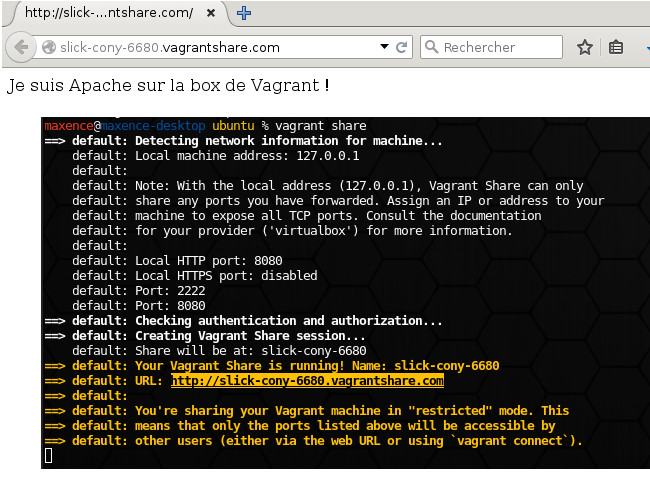
\includegraphics[width=9cm]{images_rapport/sharehttp.jpg}
        \end{center}
    \end{frame}

    \begin{frame}{Partage sur le réseau}
        \begin{center}
            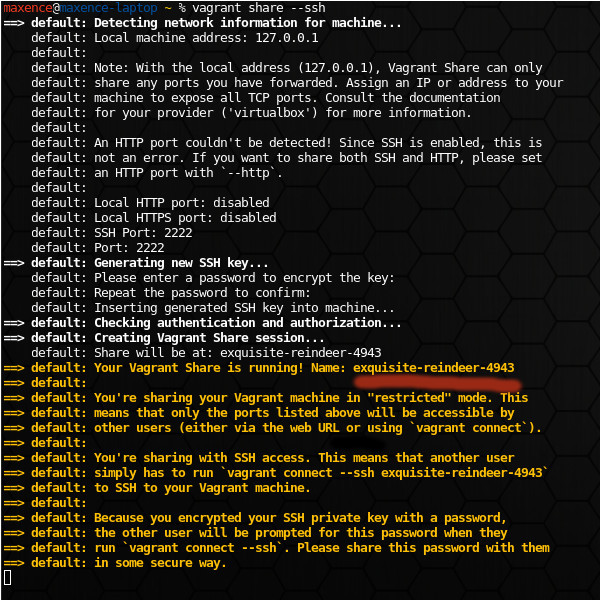
\includegraphics[width=7cm]{images_rapport/vagrantshare.jpg}
        \end{center}
    \end{frame}

    \begin{frame}{Partage sur le réseau}
        \begin{center}
            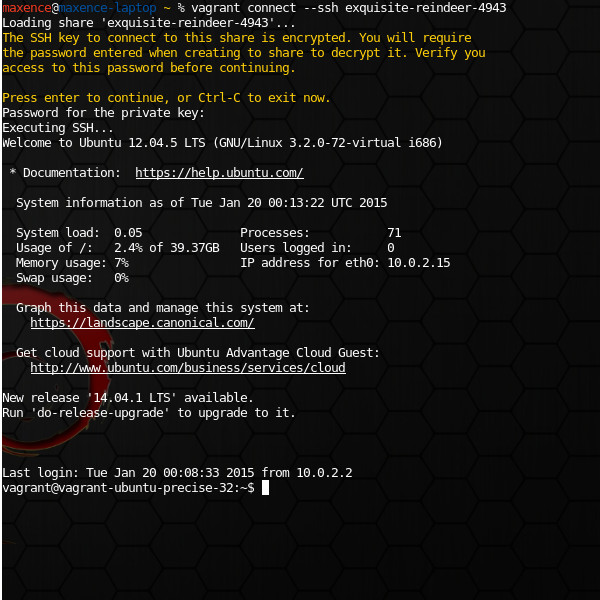
\includegraphics[width=7cm]{images_rapport/vagrantconnect.jpg}
        \end{center}
    \end{frame}

    \begin{frame}[containsverbatim]{L'environnement multi machine}
        Le but de cette fonctionnalité est de regrouper la configuration de plusieurs machines dans un seul Vagrantfile :
        \begin{minted}[fontsize=\scriptsize]{ruby}
            Vagrant.configure(2) do |config|
                config.vm.define "precise" do |precise|
                    precise.vm.box = "hashicorp/precise32"
                end
                config.vm.define "trusty", autostart: false do |trusty|
                    trusty.vm.box = "hashicorp/trusty64"
                end
            end
        \end{minted}
        \begin{alertblock}{Attention}
            Certaines commandes devront être complétées du nom de l'environnement, comme \em{vagrant ssh precise}
        \end{alertblock}
    \end{frame}

    \begin{frame}[containsverbatim]{Les provisions shell}
        Les provisions permettent d'automatiser des installations ou scripts lors de la commande vagrant up :
        \begin{minted}[fontsize=\scriptsize]{ruby}
            config.vm.provision "apache", inline: <--SHELL
                sudo apt-get update
                sudo apt-get install -y apache2
            SHELL
        \end{minted}
        \begin{itemize}
            \item{vagrant provision}
            \item{vagrant provision --provision-with apache sql}
            \item{vagrant up --no-provision}
        \end{itemize}
    \end{frame}

    \begin{frame}[containsverbatim]{Les provisions shell}
        Il est possible de combiner les provisions avec un environnement multi-machine :
        \begin{minted}[fontsize=\scriptsize]{ruby}
            config.vm.provision "mysql", type: "shell", 
                inline: "apt-get install mysql-server"
            
            config.vm.define "web" do |web|
                web.vm.provision "php", 
                    inline: "apt-get install php5"
                web.vm.provision "apache2", type: "shell", 
                    inline: "apt-get install apache2"
            end
        \end{minted}
    \end{frame}

    \begin{frame}[containsverbatim]{Les provisions file}
        La provision nommée "file" permet d'envoyer un fichier vers le système invité :
        \begin{minted}[fontsize=\scriptsize]{ruby}
        config.vm.provision "file", source: ".zshrc", destination "/home/user/.zshrc"
        \end{minted}
    \end{frame}

    \begin{frame}[containsverbatim]{Les provisions Docker}
        Les provisions Docker permettent de créer, déployer, configurer et démarrer des conteneurs : 
    \end{frame}
    
    
    
    
    
    
    
    
    
    
    
    
    
    
    
    
    
    
    
    
    
    
    
    
    
    
    
    
    
    
    
    
    
    
    
    
    
    
    
    
    % ================= Section Docker =======================
    
    \section{Docker}
    \subsection{Introduction}
    \begin{frame}
       \begin{itemize}
          \item{Développé en Go, sous licence Apache 2.0}
          \item{Créer par Salomon Hykes en Mars 2013}
          \item{Architecture légère}
          \item{}
       \end{itemize}
    \end{frame}

    \subsection{Installation}
    \begin{frame}
       \begin{itemize}
          \item{Installation rapide depuis le dépôt Debian 8}
          \item{Installation sous OS X et Windows via une machine virtuelle}
          \item{Récupération d'une image sur le dépôt Docker}
       \end{itemize}
    \end{frame}

    \subsection{Utilisation des Conteneurs}
    \begin{frame}
       \begin{itemize}
          \item{Qu'est-ce qu'un conteneur ?}
          \item{Lancer un conteneur à partir d'une image}
          \item{Déployer des outils avec le conteneur}
       \end{itemize}
       \begin{exampleblock}{}
          \em{}
       \end{exampleblock}
    \end{frame}

    \subsection{Les fichiers de configurations Dockerfile}

    \subsection{Partage et export des images Docker}
    \subsubsection{Partage par archive}
    \subsubsection{Partage par le hub de Docker}

% ================== Concurrence ========================


% ================== Conclusion =========================

\end{document}
